\documentclass{article}

\oddsidemargin 0in
 \textwidth 6.75in
 \topmargin 0in
 \textheight 8.5in
 \parindent 0em
 \parskip 2ex

\usepackage[utf8]{inputenc}
\usepackage{graphicx}
\usepackage{natbib}
% %/// librerias necesarias para generar los diagrmas de flujo ///
\usepackage{tikz}
\usetikzlibrary{shapes,arrows,chains}
% % ///////////////////////////
\usepackage[most]{tcolorbox}

\renewcommand{\figurename}{Fig.}
\newcommand{\dgC}{  $^{\circ}$C\ }

\title{Control}
\author{vargasmorenoalberto }
\date{November 2019}

\begin{document}
    
    % \section{Introducci\'{o}n}
    % Para controlar la potencia de entrada a la resistencia se utiliza un control de fase.

    \section{Principio de funcionamiento}
    \label{principio-de-funcionamiento}
    \textbf{Control por \'angulo de fase}\\
    El control de potencia en corriente alterna consiste en aplicar a la carga una porci\'on de cada semiciclo de voltaje de l\'inea de manera sim\'etrica; mientras menor es la porci\'on, menor es la potencia transferida a la carga \cite{slp}. Esta porci\'on est\'a en relaci\'on al \'angulo de fase. \\
    El control de fase es el m\'etodo m\'as com\'un para controlar potencia utilizando tiristores \cite{littelfuse}.\\

        \begin{figure}[htbp]
            \centering
            \frame{ \includegraphics[scale=0.5]{images/sineWavePhaseControl.png} }
            \caption{Onda Senoidal Mostrando principios del control de fase}
            \label{fig:formaDeOnda}
        \end{figure}
        
    En la  figura \ref{fig:formaDeOnda} se ilustra la forma de onda del voltaje de l\'inea y se muestran t\'erminos com\'unmente utilizados para describir la operaci\'on de los tiristores. El \'angulo de retardo es el tiempo durante el cual el tiristor bloquea el flujo de corriente del voltaje de l\'inea, el \'angulo de conducci\'on es el tiempo durante el cual el tiristor es activado y permite el flujo de corriente a trav\'es de la carga \cite{littelfuse}.\\
    Despu\'es de un cruce por cero el tiristor es encendido a trav\'es de una se\~nal de control recibida en la compuerta y autom\'aticmente se apaga cuando su corriente llega al valor de 0. Mientras la se\~nal de control no es recibida, el tiristor bloquea todo el flujo de corriente; este comportamiento es el mismo tanto para el semiciclo positivo como para el semiciclo negativo. Solo hay algunas limitaciones para encender el tiristor alrededor del cruce por cero, cuando la corriente no es suficiente, cuando dicha corriente es menor a la corriente de enganche del tiristor, provocando que la potencia de la carga no pueda ser regulada perfectamente de 0 a 100 \% \cite{st}.
    
    \section{Ventilador}
    El sistema de ventilaci\'on tiene dos prop\'ositos: enfriar y distribuir (forzar convecci\'on). Una soluci\'on muy simple puede ser un ventilador corriendo continuamente a toda velocidad. Aunque esta soluci\'on cumple con el prop\'osito, tiene la desventaja de consumir mucha potencia y generar mucho ruido. Un uso m\'as eficiente es ajustar la velocidad del ventilador de acuerdo a las condiciones del sistema. Resultando en un sistema de lazo cerrado, donde el ventilador intenta mantener estable las condiciones del sistema mediante el ajuste de su velocidad.\\
    
    \section{Diagrama a bloques del sistema}

        \begin{figure}[h!]
            \centering
            \frame{ \includegraphics[scale=0.5]{images/diagramaBloques.png} }
            \caption{Diagrama de bloques}
            \label{fig:bloques}
        \end{figure}
        
        \textbf{Control de fase}\\    
        El elemento principal para realizar el control de fase es el microcontrolador  MSP430G553 que controla al triac.
        La sincronizaci\'on requerida para encender el triac al mismo tiempo para cada semiciclo es provista por la detecci\'on del cruce por cero.
        El microcontrolador detecta el cruce por cero despu\'es del final de cada semiciclo de la se\~nal de entrada y ajusta el tiempo de retardo para encender el triac en relaci\'on con el porcentaje de potencia requerida.
        De manera que la fase pueda ser manipulada externamente, se usa como referencia el valor de potencia requerido.
        La fuente de alimentaci\'on para este circuito no est\'a integrada a este m\'odulo.
    
        \textbf{Ajuste de velocidad del ventilador}\\
        El sistema es realizado utilizando el microcontrolador MSP430 para controlar la velocidad del ventilador usando una salida de pwm, según sea solicitado por el control principal.\\


    \section{Descripci\'on del circuito}
    
    Se usa un triac para poder controlar la pontencia entregada al calefactor alimentado con el voltaje de l\'inea de 120 VAC. El dispositivo a cargo para activar el triac es un MOC3011. Que tiene una corriente de activaci\'on para el LED $I_{FT}$ = 10mA y capaz de tolerar, en sus terminales de salida, hasta $V_{DRM}$ = 250 V. El triac utilizado, BTA16, tiene una corriente RMS en estado encendido $I_{T}$(RMS) = 16 amps a $T_C$ = 25 $^\circ$C. La carga es un alambre de n\'iquel-cromo cubierta con acero inoxidable y rellena con \'oxido de magnesio para tener un aislamiento el\'ectrico (industrialmente denominada resistencia tubular y ampliamente utilizados para la calefacci\'on de aire), que produce temperaturas de hasta 650 $^\circ$C.\\

        \textbf{Aislamiento óptico}\\
        Para evitar sobretensiones y subidones de corriente, evitar transitorios que puedieran dañar al microcontrolador. Es tambi\'en una interfaz entre el circuito de control y la carga de potencia\\

        \textbf{Alimentación}\\
        El microcontrolador y los dispositivos electr\'onicos de esta etapa son alimentados por la fuente principal. 3.3V para el microcontrolador y 5V para los perifericos.\\

        \textbf{Detector de cruce por cero}\\
        El optoacoplador H11AA1 está diseñado para el monitoreo de señales de corriente alterna. Cuando la corriente de entrada supera la $I_F$ = 10mA, uno de los dos ledes infrarrojos enciende y permite la conducción de Colector a Emisor en el fototransistor. El fototransistor NPN está conectado en el colector a una resistencia de pullup para generar una señal invertida; esta señal de salida son los pulsos que indican al microcontrolador cuando un cruce por cero sucede.\\

        \textbf{Activación aislada del Triac}\\
        Desde el microcontrolador se envía una señal lógica al transistor que sirve como interfaz para el sistema alimentado a 5 V. Cuando se envía un uno lógico la corriente a través del led emisor del MOC3011 es suficiente para encenderlo, se permite el paso de corriente en la compuerta del triac BTA16, activando el estado de conducción.\\
        
        \textbf{Ajuste de velocidad del ventilador}\\
        La salida de pwm se aplica al ventilador a través de un transistor, que realiza la función de interfaz entre los 3.3V del microcontrolador y los 24V que alimentan el ventilador.\\

    \begin{figure}[ht]
        \centering
        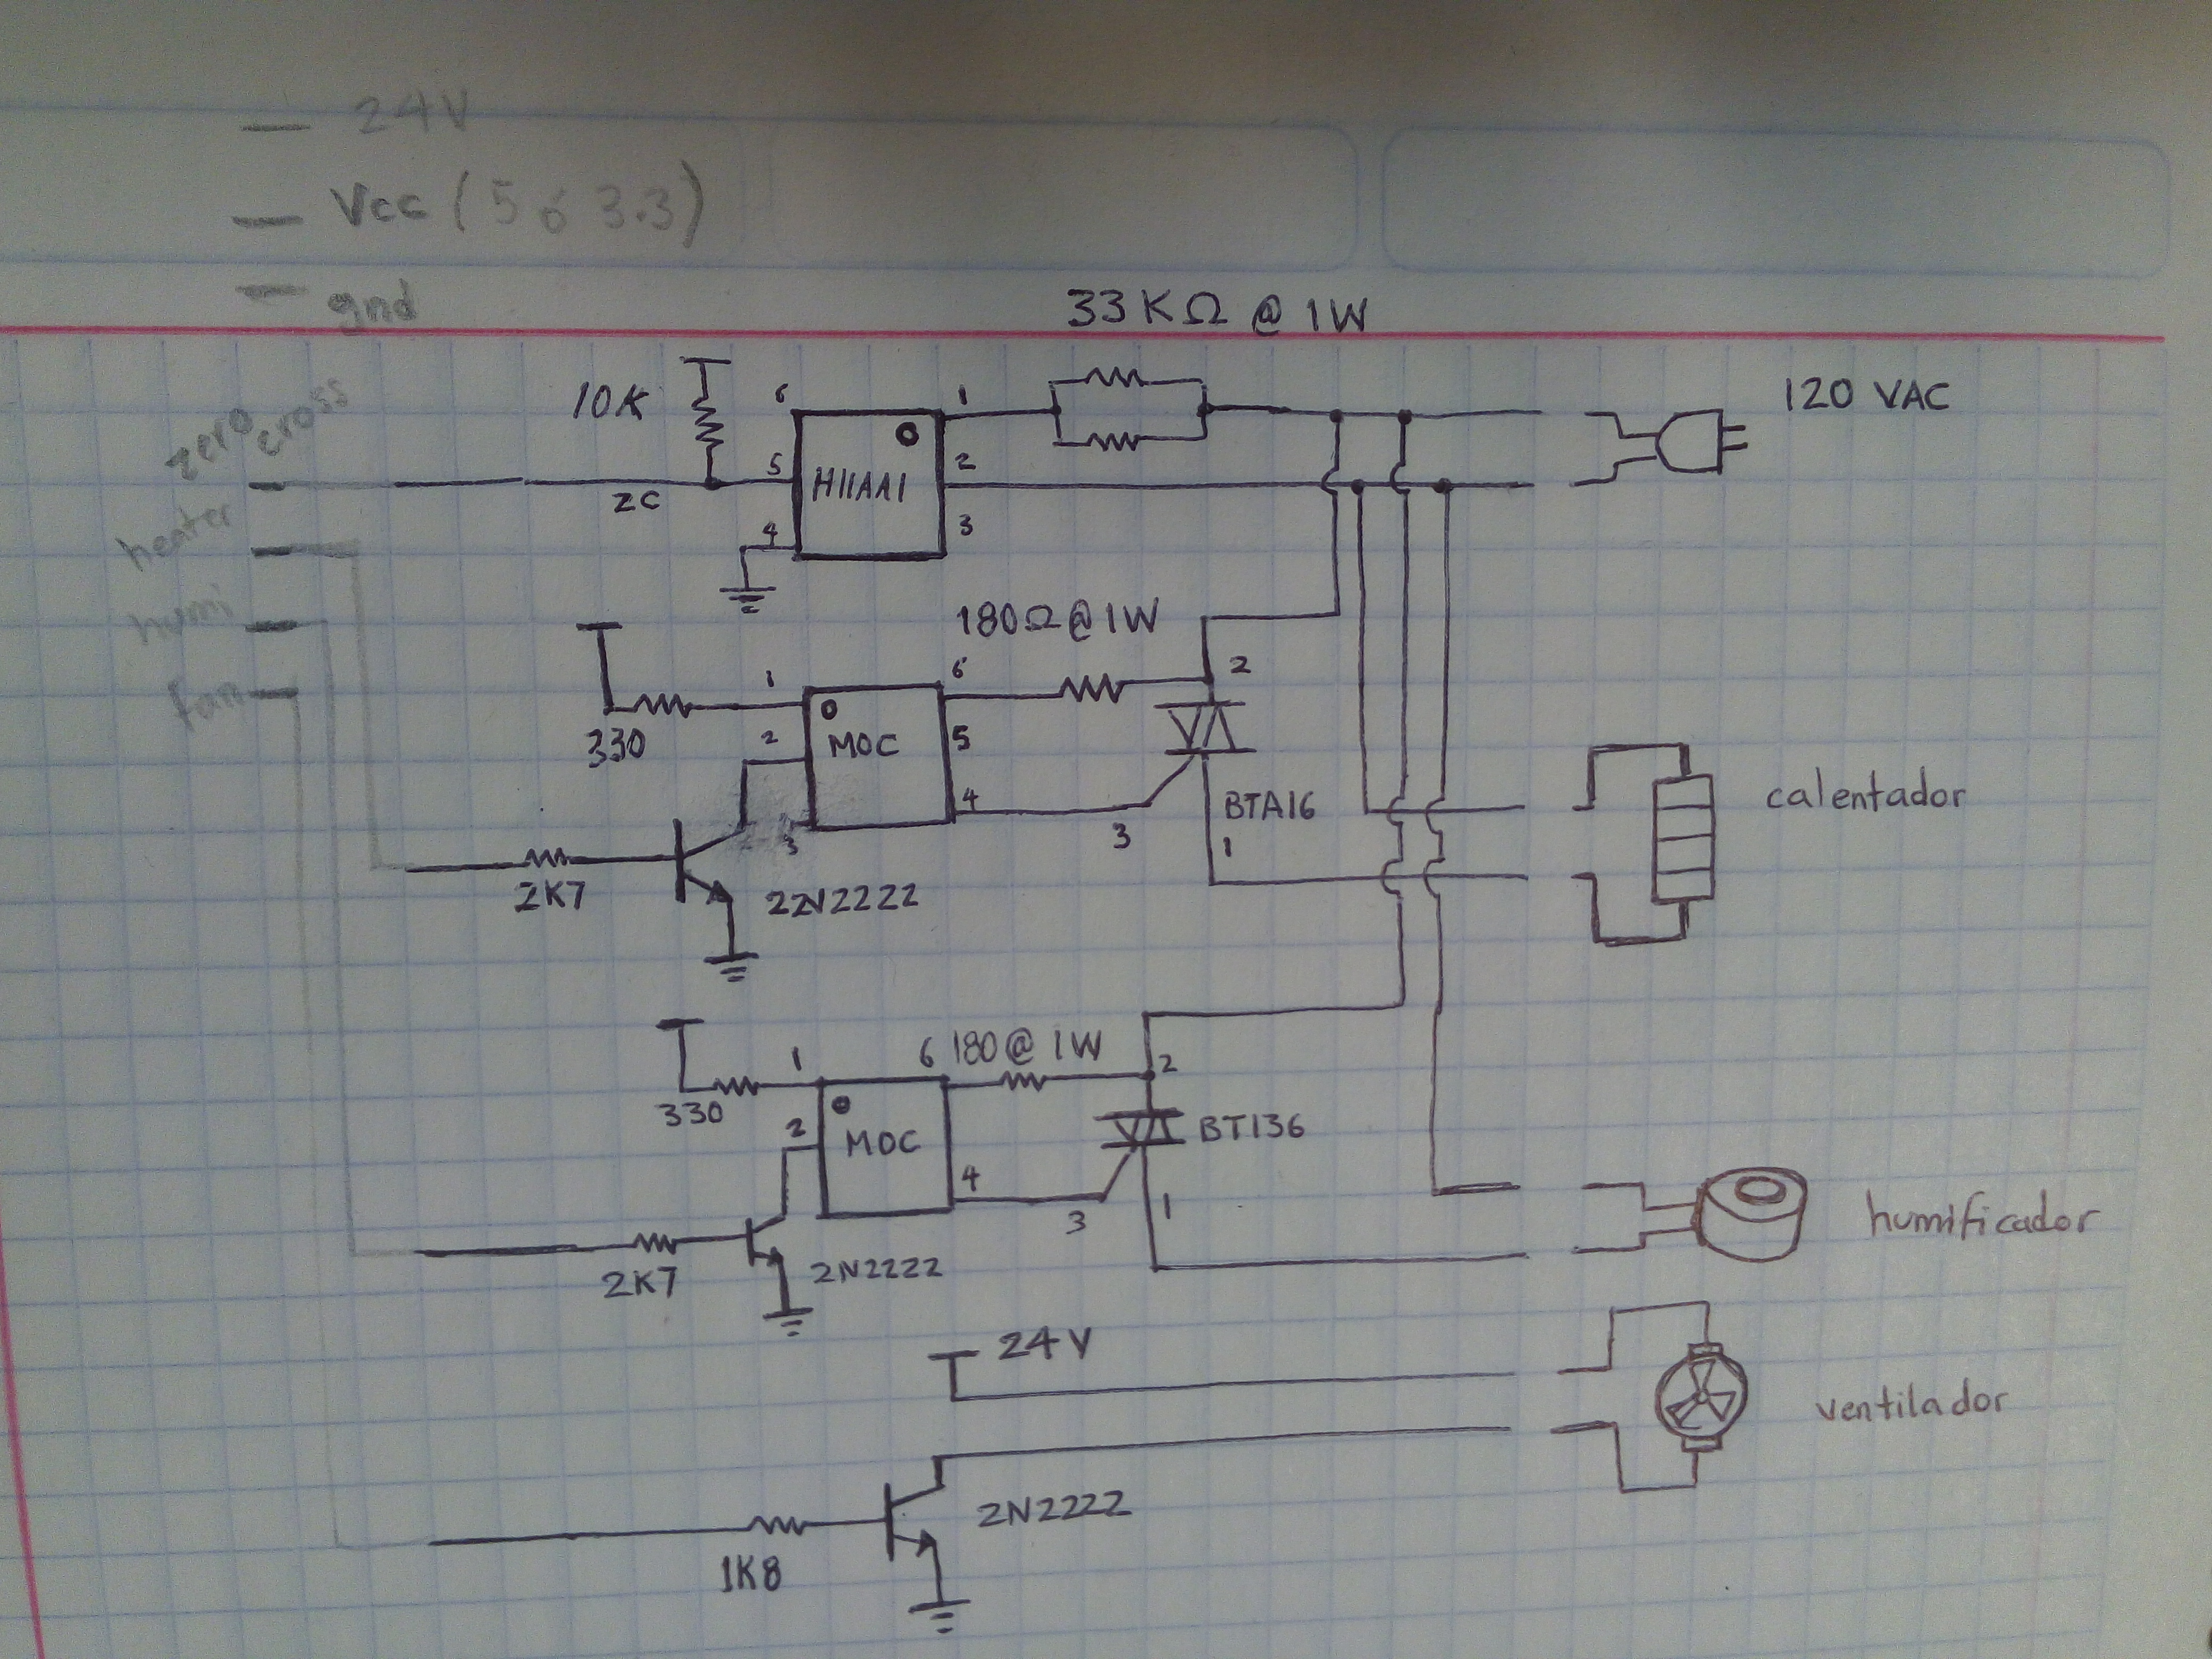
\includegraphics[scale=0.07]{images/fotos/circuito-msp.jpg}
        \caption{Esquema del circuito}
        \label{fig:esquematico}
    \end{figure}

    \section{Software}
    \textbf{CONTROL DE FASE}\\
    Una vez detectado el cruce por cero lo que se hace internamente por software mediante una conversión se calcula el tiempo de espera para activar el triac en modo de conducción.\\
    El software est\'a escrito en lenguaje C. Este est\'a compuesto de varias funciones, pero las funciones principales necesarias para la operacion apropiada del control de fase reside en: \verb|main()|, \verb|Zero_Cross_Interruption()|, \verb|TA0_ISR()|\\
    El principio de funcionamiento del TRIAC descrito en la secci\'on \ref{principio-de-funcionamiento} para controlar la resistencia calefactora es ENCENDER el TRIAC exactamente en el mismo tiempo en ambos semiciclos de la onda senoidal. El TRIAC se cierra autom\'aticamente cuando ocurre la detecci\'on del cruce por cero.\\
    La idea principal del software es sincronizar el temporizador interno del microcontrolador MSP430G2553 con los eventos de cruce por cero generados a partir de la onda senoidal del voltaje de red. El pulso que indica la ocurrencia de el cruce por cero es aplicado en el pin P1.3 el cual est\'a configurado como entrada de interrupci\'on en una configuraci\'on de pull-up.\\
    
    \textbf{AJUSTE DE VELOCIDAD DEL VENTILADOR}\\
    El software tiene 4 niveles de velocidad definidas por el sistema (estoy incluyendo: apagado). Cada nivel es representado por un valor hexadecimal asignados por conveniencia. Cada nivel de velocidad es solicitado por el control principal mediante un dato recibido por comunicación serial. Por ejemplo, si el valor 0x82 es recibido, indica que el sistema debe estar al nivel de velocidad 2. \\ \\


        \textbf{Main} \\
        Despu\'es de que el microcontrolador es encendido o reiniciado, todos los perifericos utilizados (Puertos, Temporizador y UART) son configurados en este funci\'on. Despu\'es todas las variables son inicializadas y el microcontrolador queda en un modo de bajo consumo.
        \\ \\
        \begin{figure}[ht]
            \centering
            \tcbox[ sharp corners, left=30mm,right=30mm, boxsep=5mm, boxrule=0.3mm, colback=white ]
                {   \input{ images/flowchart/mainFlowchart.tiz }    }
            \caption{Diagrama de flujo principal}
            \label{fig:my_lab}
        \end{figure}

        \textbf{Interrupci\'on por puertos} \\
        Cuando el evento de cruce por cero ocurre se genera una interrupci\'on. El funcionamiento de esta interrupci\'on es controlado en este m\'odulo por la rutina de interrupci\'on \verb|__interrupt void Zero_Cross_Interruption(void)| la cual comprueba que suceda una transici\'on de estado alto a estado bajo, en el pin 3 del puerto 1 (P1.3). Este pin es configurado como entrada de interrupci\'on que est\'a configurado como pull up. Al ocurrir la interrupci\'on la variable \verb|ZeroCross_ocurred| es encendida.\\ \\

        La funci\'on de comparaci\'on es entonces sincronizada con el evento de cruce por cero. \\ \\

        \begin{figure}[ht]
            \centering
            \tcbox [ sharp corners, left=30mm,right=30mm, boxsep=5mm, boxrule=0.3mm, colback=white ]
                {   \input{images/flowchart/port1.tiz}    }
            \caption{flujo int puertos}
            \label{fig:my_label0}
        \end{figure}

        \textbf{Interrupci\'on del temporizador} \\
        El temporizador timerA0 es configurado en modo continuo y realiza la funci\'on de ser el contador principal de tiempo. Esta interrupci\'on es manejada en la rutina de interrupci\'on \verb|TA0_ISR(void)|. Esta rutina genera la base de tiempo de 0.2ms, la activaci\'on del TRIAC. la rutina de verificaci\'on para reiniciar el contador. \\

        La rutina de interrupci\'on \verb|TA0_ISR(void)| es ejecutada cada 0.2 ms.\\

        \begin{figure}[ht]
            \centering
            \tcbox[ sharp corners, left=10mm,right=0mm, boxsep=5mm, boxrule=0.3mm, colback=white ]
            {   \input{images/flowchart/timerA0.tiz}    }
            \caption{flujo int timer}
            \label{fig:my_label1}
        \end{figure}
    \newpage

    \section{Cálculos}
    \subsection{Cruce por cero}

    Para encender los ledes infrarrojos del H11AA1 hay que satisfacer los requisitos especificados en su hoja de datos. Para superar el valor mínimo de $I_F$min = 10mA.
    
    \begin{equation}
        R_{zc}max
        =   \frac{ V_{R_{zc}} }{ I_{F}min }
        =   \frac{ V_{p} - V_{F} }{ I_{F}min }
        =   \frac{ 120 \sqrt{2}V - 1.2V }{ 10mA }
        =   16.8505 k\Omega
    \end{equation}
    
    \begin{equation}
        R_{zc}min
        =   \frac{ V_{R_{zc}} }{ I_{F}max }
        =   \frac{ V_{p} - V_{F} }{ I_{F}max }
        =   \frac{ 120 \sqrt{2}V - 1.2V }{ 50mA }
        =   3.3 k\Omega
    \end{equation}
    
    Se elige un valor cercano al valor máximo de resistencia para optimizar protección y vida útil del Led emisor.\\
    
    La potencia disipada por la resistencia limitadora está dada por:
    
    \begin{equation}
        P_{R_{zc}}   
        =   ( R_{zc} )( I_F )^2 
        =   (  16.5K\Omega )( 10mA )  
        =   1.65W
    \end{equation}
    
    En valores éstandar, 16k$\Omega$ para 2 W, sería lo ideal. Pero la variedad de valores de resistencia de potencia es restringida, como solución se propone un arreglo de resistencias. Con un arreglo paralelo de dos resistencias con valor éstandar de 33k se obtiene un valor resultante de 16.5k$\Omega$; disipando cada una 0.8425W.\\

\subsection{Disparo del Triac y el optoacoplador que le controla}
    La interfaz para el triac de potencia BTA16 es el MOC3011. Tiene una corriente de activación para el LED $I_{FT}$ de 10 mA y un voltaje de estado apagado en las terminales de salida $V_{DRM}$ de 250 V.\\
    
    Se elige un valor para $I_{FT}$ suficiente para activar y mandar la señal de activación al triac BTA16 correctamente, se eligió un valor de 15 mA.\\
    
    Un transistor NPN 2N2222 es la interfaz entre el pin de salida del microcontrolador y la entrada del optoacoplador MOC3011; en base a su hoja de datos:
    
    $V_F$ = 1.5V, $I_{FT}$ = 15mA del MOC3011;  $V_{CE(sat)}$ = 0.3V del NPN 2N2222
    
    \begin{equation}
        R_{C}min 
        =   \frac { V_{CC} - V_{F} - V_{CE(sat)} } { I_{FT} }
        =   \frac { 5V - 1.5V - 0.3V } { 15mA }
        =   213.33\Omega
    \end{equation}
     
    \begin{equation}
        P_{ R_{C} }
        =   R_{C} \cdot {I_{F}}^2
        =   (213.33\Omega) \cdot (15mA)^2
        =   47.9992mW
    \end{equation}
    
    \begin{center}
        Un valor éstandar de 330 ohm con tolerancia de 10\%, a 1/4 W es suficiente.\\
    \end{center}

    \begin{equation}
        I_{B}   
        =   \frac { I_{C} } { hFE }
        =   \frac { 15mA } { 10 }
        =   1.5mA
    \end{equation}

    \begin{equation}
        R_{B}min   
        =   \frac { Vout - V_{BE(sat)} } { I_{B} }
        =   \frac { 3.3V - 0.6V } { 1.5mA }
        =   1.8k\Omega
    \end{equation}
    
    \begin{equation}
        P_{R_{B}}
        =   R_{B} \cdot {I_{B}}^2
        =   (1.4k\Omega) \cdot (1.5mA)^2
        =   3.15mW
    \end{equation}
    
    \begin{center}
        Se eligió valor de 2.7K ohm con una tolerancia de 10\%, a 1/4 W.\\
    \end{center}
    
    \subsubsection*{Resistencia Limitadora de corriente para la compuerta}
        Esta resistencia limita la corriente pico que circula a través de la salida del optoacoplador. Su valor mínimo se calcula así:

        \begin{equation}
            R_{ }min   
            =   \frac { V_{pk}max } { I_{max} }    
            =   \frac { 170V } { 1.2A } \approx 150\Omega
        \end{equation}
        
        Por lo que se elige una resistencia, con valor éstandar, de 180 ohm para la resistencia limitadora.
        
    \subsubsection*{Disipación de potencia del TRIAC}
    Calcular la máxima salida de potencia (carga máxima) es una de las tareas más importantes en este diseño, y la capacidad de potencia depende principalmente del TRIAC que se usa. La capacidad actual del TRIAC limita la máxima salida de potencia.\\
    
    El BTA16-600V es un triac de 16 A. El triac es de tipo snubberless, por tanto no se necesitara ningún circuito de amortiguación como protección. Además de que la carga es resistiva. 
    
        \subsubsection*{Córriente en la carga}
        La potencia máxima de salida en la aplicación ( 800W ), por lo que el flujo de coriene RMS a través del TRIAC para un 800 W es 6.66 A.

            \begin{equation}
                I   
                =   \frac{ P_{LOAD} }{ V_{IN} }  
                =   \frac{800}{120}    
                =   6.6666 A
            \end{equation}

        
\subsection{Ventilador}
    El ventilador se alimenta a 24 Vdc. Un simple transistor BJT sirve de interfaz entre la salida del microcontrolador a 3.3 V y los 24 V. Se eligió un 2N2222, cuyas características son: $V_{CE(sat)}$ = 0.3 V del NPN 2N2222; y teniendo en cuenta que I$_{C}$ = I$_{fan}$max = 0.25 Amps.
    
    \begin{equation}
        R_{C} 
        =   \frac { V_{CC} - V_{fan} - V_{CE(sat)} } { I_{fan} }
        =   \frac { 24V - 24V - 0.3V } { 250 mA }
        \approx   0 \Omega
    \end{equation}
    
    \begin{center}
        La caída de voltaje en el ventilador es aproximadamente el total de la fuente de alimentación y la caída de voltaje colector-emisor es despreciable, por tanto no es necesario utilizar una resistencia limitadora de corriente para la carga.\\
    \end{center}
    
    \begin{equation}
        I_{B}   
        =   \frac { I_{C} } { hFE }
        =   \frac { 250mA } { 10 }
        =   25mA
    \end{equation}

    \begin{equation}
        R_{B}   
        =   \frac { Vout - V_{BE(sat)} } { I_{B} }
        =   \frac { 3.3V - 0.6V } { 25 mA }
        =   1.8k\Omega
    \end{equation}
    
    \begin{equation}
        P_{R_{B}}
        =   R_{B} \cdot {I_{B}}^2
        =   (1.4k\Omega) \cdot (1.5mA)^2
        =   3.15mW
    \end{equation}
    
    \begin{center}
        Se elige un valor de 2.7K ohm con una tolerancia de 10\%, a 1/4 W.\\
    \end{center}
    

    \bibliographystyle{ieeetr}
    \bibliography{referencias}

\end{document}
